% Etiquetas que uso para editar en la próxima iteración:
% FALTA, VER


\chapter{ \textsc{ Verificación Formal } }\label{verificacion}

Como aclaramos en el capítulo \ref{diseñoDigital}, el correcto funcionamiento del circuito se garantiza por medio de la verificación formal de las propiedades de la suma. 

Nuestro flujo para esta etapa tiene que ver con la verificación de propiedades que se denominan \emph{safety properties}. Estas  son propiedades que se mantienen como verdaderas siempre (o lo que es equivalente, nunca son falsas). En Lava escribimos estas propiedades de la misma forma en que escribimos los circuitos, inclusive utilizando otros circuitos que nos sirvan para expresar una condición. Esto se verá con mas claridad cuando avancemos con la verificación. Entonces, la pregunta que estamos haciendo para verificar cualquier propiedad descrita de esta forma es:  ¿Este circuito de verificación siempre tiene como salida el estado \verb.True. sin importar cuales son las entradas? Para responder esta pregunta, en Lava usamos la operación \verb.verify..

Este proceso funciona asi: Tal como podemos generar un netlist VHDL (o la simulación) a partir de la descripción del circuito, también podemos generar una fórmula lógica que representa al circuito. Esta fórmula lógica se la damos a un probador de teorema externo que nos probará (o desaprobará) la validez de la fórmula. El probador externo que usaremos es MiniSAT\cite{minisat}\footnote{Minisat es un programa que resuelve problemas conocidos como \emph{Boolean satisfiability problem (\gls{sat})}, o directamente \emph{SAT solver}.}.

\section{Modelo de referencia}
A los fines de la verificación, usaremos un sumador de referencia \verb.adder. bien simple, en el cual podamos probar todas las propiedades de la suma, para luego hacer un chequeo de equivalencia lógica (LEC por sus siglas en inglés) entre el sumador de referencia y el sumador que queremos implementar. Esto es conveniente porque es una gran ventaja (desde el punto de vista de tiempo de cálculo) hacer todas las pruebas sobre circuitos mas simples (pequeños), para luego realizar una sola comprobación de equivalencia lógica entre este circuito simple y el circuito diseñado, garantizando así que si todas las propiedades se cumplen en uno, también se cumplen en el otro.

\section{Verificación de las Propiedades}
\subsection{Propiedades de la suma}
La suma tiene las siguientes propiedades:
\begin{itemize}
\item Asociativa
\item Conmutativa
\item Existencia del elemento neutro cero.
\end{itemize}

\subsection{Descripción de las propiedades en el Ripple Carry Adder}
Debido a que nuestro sumador de Brent-Kung asume que el acarreo de entrada es cero, debemos modificar nuestro sumador de referencia (un Ripple Carry Adder) para que desprecie el acarreo de entrada. Por lo tanto describimos nuevamente una versión del Ripple Carry de la siguiente forma:

%TODO Revisar porque no entiendo si esta bien o mal esta version del sumador.

\begin{lstlisting}
adder2 ([],[]) = []
adder2 (a:as, b:bs) = sum:sums
  where
    (sum, carry)     = halfAdd (a, b)
    (sums, carryOut) = adder2 (carry, (as, bs))
\end{lstlisting}

\subsubsection{Propiedad Conmutativa}
Ahora declaramos la propiedad conmutativa de la suma de la siguiente forma:
\begin{verbatim}
prop_AdderCommutative (as, bs) = ok
   where
      out1 = adder2 (as, bs)
      out2 = adder2 (bs, as)
      ok   = out1 <==> out2
\end{verbatim}
\noindent Notar que el operador {\footnotesize\verb|<==>|} es la versión infija de una función que mapea dos listas a la compuerta {\footnotesize\verb|xnor2|}, la cual es la operación de equivalencia lógica. Como es muy difícil verificar automáticamente para cualquier tamaño, definimos una nueva propiedad que incluye el tamaño del circuito a ser verificado:
\begin{verbatim}
prop_AdderCommutative_ForSize n =
   forAll (list n) $ \as ->
     forAll (list n) $ \bs ->
       prop_AdderCommutative (as, bs)
\end{verbatim}

\noindent Luego hacemos la verificación corriendo Minisat
 desde Lava, dando el tamaño del sumador:
\begin{lstlisting}
minisat (prop_AdderCommutative_ForSize 32)
\end{lstlisting}

\noindent Si nuestro circuito está correctamente diseñado, tenemos:
{\footnotesize
\begin{verbatim}
Minisat: ... (t=0.00system) Valid.
\end{verbatim}
}

\noindent De otro modo, podemos tener uno de estos resultados:

{\footnotesize
\begin{verbatim}
Minisat: ... (t=0.00system) Falsifiable.
Minisat: ... (t=0.00system) Inderterminate.
\end{verbatim}
}

\subsubsection{Propiedad Asociativa}
\noindent La propiedad Asociativa la declaramos como:
{\footnotesize
\begin{verbatim}
prop_AdderAssociative (as, bs, cs) = ok
   where
      out1 = adder2 (adder2 (as, bs), cs)
      out2 = adder2 (as, adder2 (bs, cs))
      ok   = out1 <==> out2
\end{verbatim}
}

\subsubsection{Existencia del Elemento Neutro}
\noindent Para verificar que el cero es el elemento neutro de la adición, necesitamos escribir un poco mas de lógica al circuito para transformar uno de los operandos a cero:

\begin{figure}[h]
  \centering
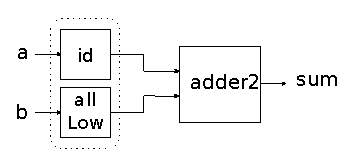
\includegraphics[scale=1]{figuras/addZero.eps}
  \caption{Circuito que nos sirve para describir la suma del elemento neutro}
\end{figure}


\begin{lstlisting}
alwaysLow :: [Signal Bool] -> [Signal Bool]
alwaysLow (as) = [low | n <- [1..n]]
   where
      n = length as

addZero = (id -|- alwaysLow) ->- adder2
-- id es la funcion identidad
\end{lstlisting}
\noindent Y la verificación de esta propiedad en el circuito:
{\footnotesize
\begin{verbatim}
prop_AdderZero (as,bs) = ok
   where
      out = addZero (as, bs)
      ok   = out <==> as
\end{verbatim}
}


\subsection{Equivalencia lógica entre el modelo de referencia y los sumadores de Brent-Kung y Sklansky}
Finalmente, hacemos la equivalencia lógica entre los dos circuitos: {\footnotesize\verb|fastAdd|} (el BKA) y {\footnotesize\verb|adder2|} (el RCA). Eso se declara en Lava de la siguiente forma:
{\footnotesize
\begin{verbatim}
prop_Equivalent adder2 fastadd a = ok
   where
      out1 = adder2   a
      out2 = fastadd a
      ok   = out1 <==> out2
\end{verbatim}
}
Y lanzamos el minisat desde Lava:
{\footnotesize
\begin{verbatim}
Minisat: ... (t=0.00system) Valid.
\end{verbatim}
}
